\documentclass[10pt]{beamer}

\usepackage{graphicx}
\usepackage{mathtools}
\usepackage{subcaption}
\usepackage{xcolor}
\usepackage{ragged2e}
\usepackage{array}
\usepackage{tikz}

\usetheme{CambridgeUS}
\usecolortheme{dolphin}
\usefonttheme{professionalfonts}

\usepackage{natbib}
\usepackage{hyperref}

% ------------------------------------------------------------
% Colors
% ------------------------------------------------------------
\definecolor{myNewColorA}{RGB}{126,12,110}
\definecolor{myNewColorB}{RGB}{165,85,154}
\definecolor{myNewColorC}{RGB}{204,158,197}

\setbeamercolor*{palette primary}{bg=myNewColorC}
\setbeamercolor*{palette secondary}{bg=myNewColorB, fg=white}
\setbeamercolor*{palette tertiary}{bg=myNewColorA, fg=white}
\setbeamercolor*{titlelike}{fg=myNewColorA}
\setbeamercolor*{title}{bg=myNewColorA, fg=white}
\setbeamercolor*{item}{fg=myNewColorA}
\setbeamercolor*{caption name}{fg=myNewColorA}
\setbeamercolor{block title}{bg=white, fg=myNewColorB}
\setbeamercolor{block body}{bg=white, fg=black}

% ------------------------------------------------------------
% Title metadata
% ------------------------------------------------------------
\titlegraphic{
\includegraphics[height=1.5cm]{vu_logo.png}}

\setbeamerfont{title}{size=\large}
\setbeamerfont{subtitle}{size=\small}
\setbeamerfont{author}{size=\small}
\setbeamerfont{date}{size=\small}
\setbeamerfont{institute}{size=\small}

\title[Vilnius University]{Shadow Fleet Detection}
\author{Tomas Giedraitis \and Jonas Adomaitis \and Gedas Beržinskas}
\institute{Vilnius University\\Faculty of Mathematics and Informatics}
\date{2026-04-09}

% ------------------------------------------------------------
% Small helpers
% ------------------------------------------------------------
\newcommand{\metricbox}[3]{
  \begin{beamercolorbox}[wd=\linewidth,sep=6pt,rounded=true,shadow=true]{block body}
    {\color{myNewColorB}\Large #1}\\[2pt]
    {\small\textbf{#2}}\\[1pt]
    {\scriptsize #3}
  \end{beamercolorbox}
}


\newcommand{\tocitem}[2]{%
  \noindent
  \begin{tikzpicture}[baseline=(n.base)]
    \node[
      circle,
      shade,
      ball color=myNewColorA,
      text=white,
      font=\bfseries\small,
      inner sep=1.8pt
    ] (n) {#1};
  \end{tikzpicture}%
  \hspace{0.75em}#2\par
}

% ------------------------------------------------------------
\begin{document}
% ------------------------------------------------------------

\frame{\titlepage}

% ------------------------------------------------------------
\begin{frame}{Contents}
\small

\vspace{6pt}

\tocitem{1}{Data}

\vspace{15pt}

\tocitem{2}{Low-Memory Partitioning}

\vspace{15pt}

\tocitem{3}{Shadow Fleet Analytics}

\vspace{15pt}

\tocitem{4}{Speedup Analysis}

\vspace{15pt}

\tocitem{5}{Real-World Geographical Map}

\vspace{15pt}

\tocitem{6}{Architecture}

\end{frame}

% ------------------------------------------------------------
\begin{frame}[t]{Data}

\begin{itemize}
  \item This dataset contains Danish AIS data from August 13th to 14th, 2025.
  \item Files processed: \texttt{aisdk-2025-08-13.csv} (5.4 GB) and
        \texttt{aisdk-2025-08-14.csv} (5.6 GB).
  \item Total rows: \(\sim\)64 million.
\end{itemize}

\vspace{10pt}

\begin{columns}[T,onlytextwidth]
  \begin{column}{0.32\textwidth}
    \metricbox{\(\sim\)26M}{rows/day}{Class A vessels}
  \end{column}
  \begin{column}{0.32\textwidth}
    \metricbox{15}{cores}{Shard workers}
  \end{column}
  \begin{column}{0.32\textwidth}
    \metricbox{A \(\cdot\) B \(\cdot\) C \(\cdot\) D}{anomaly types}{Detection categories}
  \end{column}
\end{columns}

\end{frame}

% ------------------------------------------------------------
\begin{frame}[t]{Low-Memory Partitioning \& Dirty Data Handling}

\begin{columns}[T, totalwidth=\textwidth]

  \begin{column}{0.48\textwidth}
    \textbf{\small Pipeline}\\[3pt]
    \begin{enumerate}\small
      \item \textbf{csv.reader} line-by-line\\
            {\footnotesize No \texttt{pandas.read\_csv()} -- pure Python generator}
      \item \textbf{parsing.py} filters\\
            {\footnotesize Class A only \(\cdot\) invalid MMSI \(\cdot\) bad coords}
      \item \textbf{hash(MMSI) \% N} shards\\
            {\footnotesize All pings for one ship \(\to\) same shard file}
      \item \textbf{Flush} buffer when full\\
            {\footnotesize Peak RAM \(\leq\) workers \(\times\) chunk\_size \(\times\) \(\sim\)100 B}
      \item \textbf{Output:} \texttt{ais\_shard\_*.csv}\\
            {\footnotesize 15 files on disk, processed in parallel}
    \end{enumerate}
  \end{column}

  \begin{column}{0.48\textwidth}
    \textbf{\small Dirty Data -- Filtered Out}\\[3pt]
    \begin{itemize}\footnotesize
      \item Non-Class A (Class B, AtoN, Base Station, SAR)
      \item MMSI 000000000 / 111111111 / 123456789
      \item All-same-digit MMSIs (unconfigured transponders)
      \item AIS sentinel coordinates (\(91^\circ, 0^\circ\))
      \item Always-stationary ships (SOG = 0 everywhere)
    \end{itemize}

    \vspace{2pt}
    \textbf{\small Two-Day Continuity}\\[2pt]
    {\footnotesize
    Both CSVs are processed together.\\
    Shards are sorted chronologically, so gaps spanning midnight\\
    (Aug 13\(\to\)14) are detected as one continuous event.}

    \vspace{2pt}
    {\footnotesize
    \textbf{Peak RAM:}
    \(15 \times 50{,}000 \times 100\,\text{B} \approx 75\,\text{MB} \ll 1\,\text{GB/core}\)}
  \end{column}

\end{columns}
\end{frame}

% ------------------------------------------------------------
\begin{frame}[t]{Shadow Fleet Analytics}

\definecolor{anomalyA}{RGB}{40,190,190}
\definecolor{anomalyB}{RGB}{225,180,60}
\definecolor{anomalyC}{RGB}{230,85,85}
\definecolor{anomalyD}{RGB}{165,130,245}

\begin{columns}[T, totalwidth=\textwidth]

  \begin{column}{0.48\textwidth}
    \textbf{\textcolor{anomalyA}{A} \quad Going Dark}\\[2pt]
    {\footnotesize\textcolor{anomalyA}{\textbf{Gap \(> 4\) h + implied speed \(> 1\) kt}}}\\[3pt]
    {\footnotesize
      Detected in \texttt{detect.py} per MMSI shard.\\
      Haversine distance / gap hours = implied speed.
    }

    \vspace{9pt}

    \textbf{\textcolor{anomalyC}{C} \quad Draft Changes at Sea}\\[2pt]
    {\footnotesize\textcolor{anomalyC}{\textbf{Draught change \(> 5\%\) during blackout \(> 2\) h}}}\\[3pt]
    {\footnotesize
      Compares draught values across AIS gaps.\\
      Indicates illegal cargo transfer at sea.
    }
  \end{column}

  \begin{column}{0.48\textwidth}
    \textbf{\textcolor{anomalyB}{B} \quad Loitering / Transfer}\\[2pt]
    {\footnotesize\textcolor{anomalyB}{\textbf{Distance \(< 500\) m \(\cdot\) SOG \(< 1\) kt \(\cdot\) Duration \(> 2\) h}}}\\[3pt]
    {\footnotesize
      Separate \texttt{loiter.py} module.\\
      Bounding-box pre-filter \(\to\) exact Haversine.
    }

    \vspace{9pt}

    \textbf{\textcolor{anomalyD}{D} \quad Identity Cloning}\\[2pt]
    {\footnotesize\textcolor{anomalyD}{\textbf{Implied speed \(> 60\) kt \(\cdot\) Sustained \(> 10\) min}}}\\[3pt]
    {\footnotesize
      Zigzag pattern across two pings = two ships\\
      broadcasting the same stolen MMSI.
    }
  \end{column}

\end{columns}

\vspace{18pt}
\begin{beamercolorbox}[sep=4pt, center, rounded=true]{title}
  \footnotesize\textbf{DFSI = (Max Gap Hours / 2) + (Largest Impossible Jump NM / 10) + (C \(\times\) 15)}
\end{beamercolorbox}

\end{frame}

% ------------------------------------------------------------
\begin{frame}[t]{Speedup Analysis \& Memory Profiling}

\begin{columns}[T,onlytextwidth]

  \begin{column}{0.64\textwidth}
    \centering
    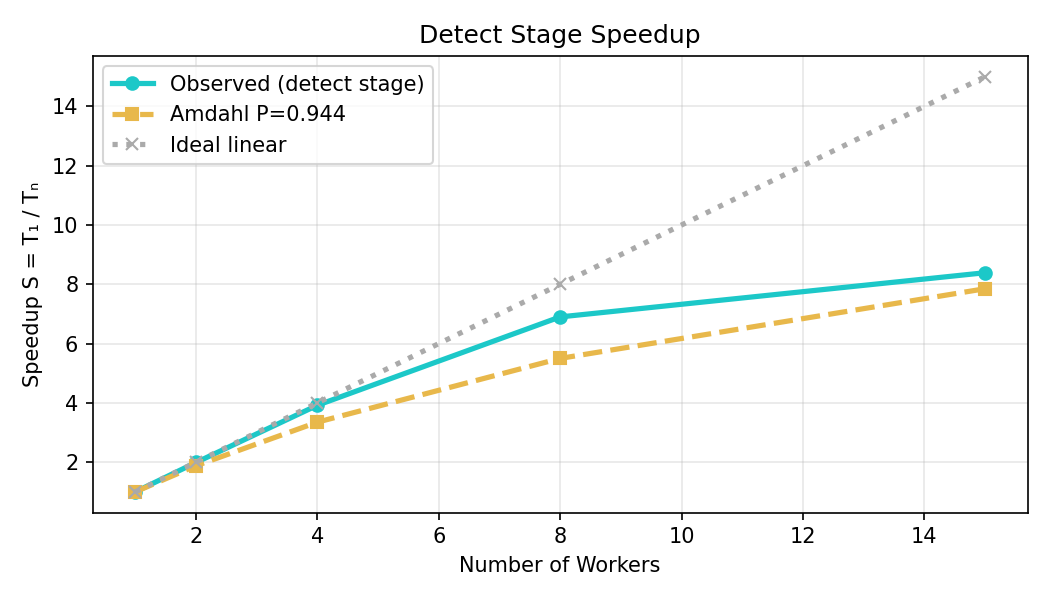
\includegraphics[width=\linewidth,height=0.36\textheight,keepaspectratio]{detect_stage_speedups_graph_hotfix.png}

    {\tiny\makebox[\linewidth][c]{Overall pipeline: \(1.13\times\) \quad \(\mid\) \quad Detect stage: \(S = 8.39\times\) \quad \(\mid\) \quad \(P \approx 0.944\)}}
    \vspace{0.5pt}
    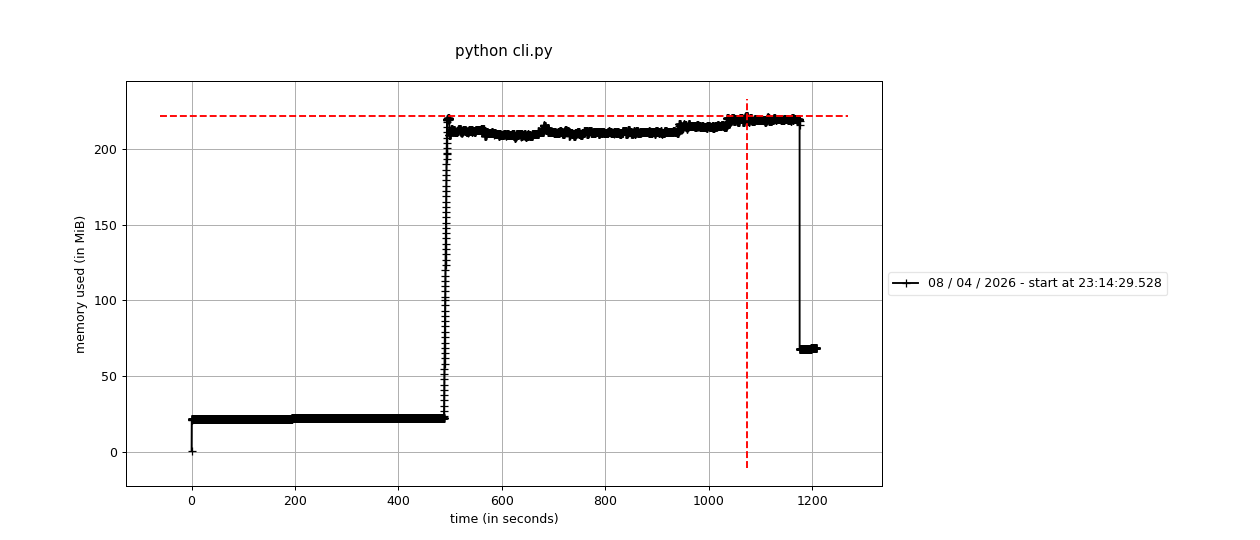
\includegraphics[width=0.98\linewidth,height=0.35\textheight]{mprof_RAM_graph.png}
  \end{column}

  \begin{column}{0.33\textwidth}
    \begin{block}{245.1 s}
      \small \textbf{Sequential detect}\\
      \scriptsize 1 worker \(\cdot\) 5\,153 vessels
    \end{block}

    \vspace{1pt}

    \begin{block}{29.2 s}
      \small \textbf{Parallel detect}\\
      \scriptsize 15 workers \(\cdot\) \texttt{imap\_unordered}
    \end{block}

    \vspace{1pt}

    \begin{block}{\(S = 8.39\times\)}
      \small \textbf{Detect speedup}\\
      \scriptsize Overall pipeline \(S = 1.13\times\)
    \end{block}

    \vspace{1pt}

    \begin{block}{\(\sim\)220 MiB}
      \small \textbf{Peak RAM}\\
      \scriptsize 1.4\% of 16 GiB limit
    \end{block}
  \end{column}

\end{columns}

\vspace{0pt}
\begin{beamercolorbox}[sep=1pt,center,rounded=true]{title}
\tiny
\textbf{Chunk-size:} 10k = 1183 s \(\cdot\) 50k = 1201 s \(\cdot\) 100k = 1213 s\\
50k chosen as best balance of flush overhead and memory use.
\end{beamercolorbox}

\end{frame}

% ------------------------------------------------------------
\begin{frame}[t]{Real-World Geographical Map}

\centering
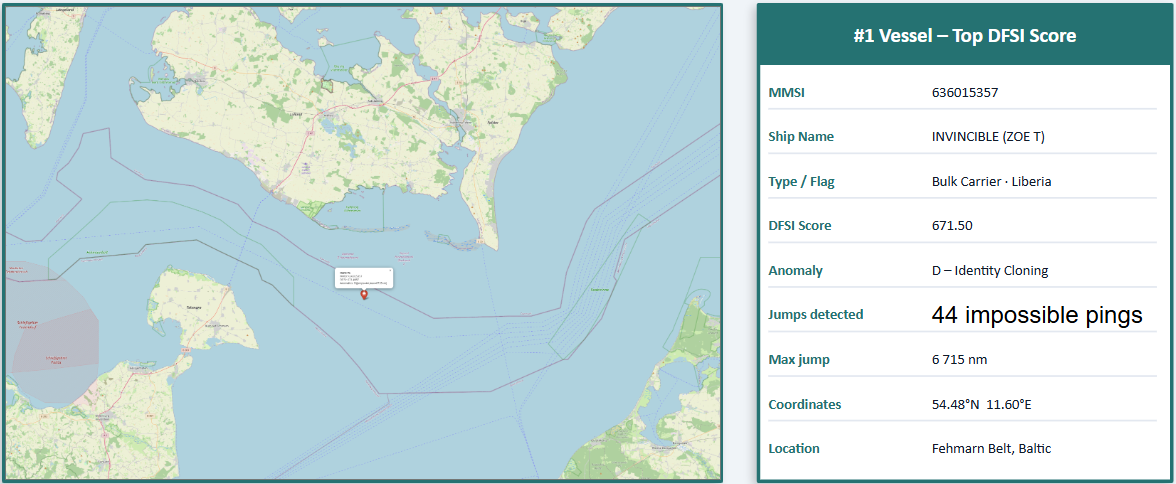
\includegraphics[width=\textwidth,height=0.72\textheight,keepaspectratio]{real_world_geo_map_with_table.png}

\vspace{3pt}
\begin{beamercolorbox}[sep=3pt,rounded=true,wd=\textwidth]{title}
\scriptsize
\textbf{Location:} Fehmarn Belt -- primary gateway between the Baltic Sea and North Sea, through which vessels exiting Russian Baltic ports must pass.

\vspace{9pt}

\textbf{Finding:} INVINCIBLE detected here with 44 impossible pings spanning 6\,715 nm, suggesting identity cloning to mask cargo movements between
sanctioned Russian ports and Western markets.
\end{beamercolorbox}

\end{frame}

% ------------------------------------------------------------
\begin{frame}[t]{Architecture}

\begin{center}
\scriptsize
\texttt{cli.py} \(\rightarrow\)
\texttt{pipeline.py} \(\rightarrow\)
\texttt{partition.py/parsing.py} \(\rightarrow\)
\texttt{detect.py (\(\times\)15)} \(\rightarrow\)
\texttt{loiter.py} \(\rightarrow\)
\texttt{scoring.py}
\end{center}

\vspace{4pt}

\begin{columns}[T,onlytextwidth]
  \begin{column}{0.49\textwidth}
    \begin{block}{\texttt{pipeline.py:44}}
      \scriptsize\texttt{pool.imap\_unordered(process\_shard, shard\_paths)}\\[3pt]
      \footnotesize Distributes shards across Pool workers; results stream back as soon as any worker finishes.
    \end{block}
  \end{column}

  \begin{column}{0.49\textwidth}
    \begin{block}{\texttt{partition.py:85}}
      \scriptsize\texttt{\_shard\_id = hash(mmsi) \% num\_shards}\\[3pt]
      \footnotesize All pings for one MMSI land in the same shard; no cross-shard joins needed.
    \end{block}
  \end{column}
\end{columns}

\vspace{3pt}

\begin{columns}[T,onlytextwidth]
  \begin{column}{0.49\textwidth}
    \begin{block}{\texttt{detect.py:60}}
      \scriptsize\texttt{speed = haversine\_nm(...) / gap\_hours}\\[3pt]
      \footnotesize If gap \(> 4\) h but speed \(> 1\) kt, flag Anomaly A.
    \end{block}
  \end{column}

  \begin{column}{0.49\textwidth}
    \begin{block}{\texttt{loiter.py:72}}
      \scriptsize\texttt{within\_bbox(b.avg\_lat, b.avg\_lon, bbox)}\\
      \scriptsize\texttt{\(\rightarrow\) haversine\_metres()}\\[3pt]
      \footnotesize Bounding-box pre-filter removes distant vessels before exact Haversine check.
    \end{block}
  \end{column}
\end{columns}

\end{frame}

% ------------------------------------------------------------
\begin{frame}
\textcolor{myNewColorA}{\Huge{\centerline{Thank you for your time!}}}
\end{frame}

% ------------------------------------------------------------
\end{document}
